\documentclass[12pt,a4paper]{article}
\usepackage[utf8]{inputenc}
\usepackage[english]{babel}
\usepackage{graphicx}
\author{Madhur Singhal\\2015CS10235}

\title{Parallel Convex Hull}
\date{26 February, 2018}
\begin{document}
\maketitle
\section{Introduction}
The convex hull or convex envelope of a set X of points in the Euclidean plane or in a Euclidean space (or, more generally, in an affine space over the reals) is the smallest convex set that contains X. Intuitively it is the set of boundary points in a given set of points, that is a surface made from joining In this assignment we implement the quick hull algorithm to solve the problem of finding the convex hull of a set of points using C++ and OpenMP.
\section{Algorithm}
The algorithm used by me is presented below.
\begin{enumerate}

   \item We find the point with minimum x-coordinate lets say, min\_x and similarly the point with maximum x-coordinate, max\_x. These are guaranteed to be in the convex hull.
 \item   Make a line joining these two points, say L. This line will divide the the whole set into two parts. We enable nested parallelism in openmp and use sections to assign the two parts to separate threads.
    \item Each thread finds the point with maximum distance from the line L. P forms a triangle with the points min\_x, max\_x. It is clear that the points residing inside this triangle can never be the part of convex hull. Wedistinguish the direction by comparing the sign of the distance from the other point.
    \item The above step divides the problem into two sub-problems. The line joining the points P and min\_x and the line joining the points P and max\_x are new lines and the points residing outside the triangle is a new set of points.  We solve the further suproblems recursively using new threads as needed. We repeat these steps until there is no point on the desired side of the line after which we add the end points of this line to the convex hull.

\end{enumerate}
\section{Design Decisions}
I opted to use task level parallelism (albeit without the OpenMP task primitive) for this task. It was clear that the recursive calls to quickhull were independent of each other and thus could be executed simultaneously. I used a std::set to store the result so that duplicate points are not added and utilized an OpenMP critical section at the portion where points are added to the set since standard library structures are not thread safe. Nested Parallelism using the omp\_set\_nested function was helpful in distributing the load across the threads. OpenMP sections were used inside a parallel block to enable different threads to execute different recursive calls.
\section{Analysis}
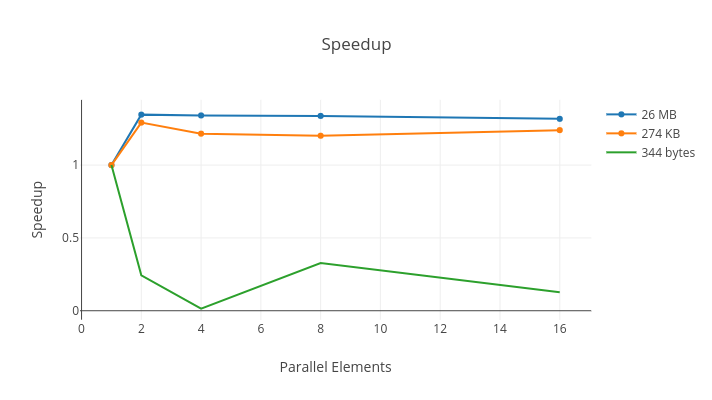
\includegraphics[scale=0.52]{spd2}\\
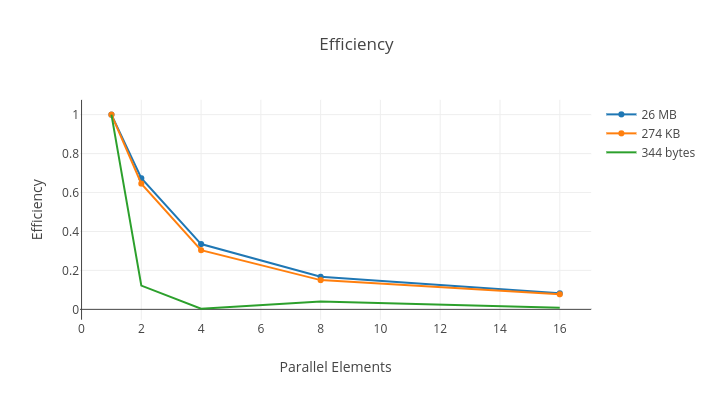
\includegraphics[scale=0.52]{eff2}
I ran the program on various sizes of input files and plotted the results. As can be seen speedup saturates at 2-4 processing elements because of the computer I am running this on. The smallest example actually results in less than one speedup since thread creation overhead dominates.\section{Conclusion}
Thus our parallel implementation performs better than the serial one in this case too. A speedup of 1.35 seems to be the best value we get.
\end{document}